% --------------------------------------------------------------------- %
% Modelo adaptado pelo aluno voluntário João Antonio Teixeira Sucupira  %
% Supervisão do Prof. Daniel Fernando Pigatto                           %
% Programa de Pós-graduação em Computação Aplicada (PPGCA)              %
% Universidade Tecnológica Federal do Paraná (UTFPR)                    %
% --------------------------------------------------------------------- %
%pdflatex -synctex=1 -interaction=nonstopmode -shell-escape %.tex
\documentclass{if-beamer}

% --------------------------------------------------- %
%                  Presentation info	              %
% --------------------------------------------------- %
\title[PPGCA -- UTFPR Curitiba]{\textbf{O USO DE LOGS NO ENSINO DE PROGRAMAÇÃO}}
\subtitle{Universidade Tecnológica Federal do Paraná}
\author[Gilmar Gomes do Nascimento]{\large \negrito{Gilmar Gomes do Nascimento}}
\institute[UTFPR-CT]{
    \small \textit{Universidade Tecnológica Federal do Paraná} \\
    \textit{Programa de Pós-Graduação em Computação Aplicada}
}
\date{\today}
\logo{

\includegraphics[scale=.15, clip]{figuras/logoPPGCA.png}
}
\subject{Presentation subject} % metadata
%trim={<left> <lower> <right> <upper>}
\graphicspath{{figuras/}}
% --------------------------------------------------- %
%                    Title + Schedule                 %
% --------------------------------------------------- %

\begin{document}

\begin{frame}
  \titlepage
\end{frame}

\begin{frame}{Programação}
  \tableofcontents
\end{frame}

% --------------------------------------------------- %
%                      Presentation                   %
% --------------------------------------------------- %

%%%%%%%%%%%%%%%%%%%%%%%%%%%%%%%%%%%%%%%%%%%%%%%%%%%%%%%%%%%%%

\section{Orientadores}
\begin{frame}{Orientadores}
\begin{columns}
        % Column 1: Name
        \begin{column}{0.5\textwidth}
            \centering
            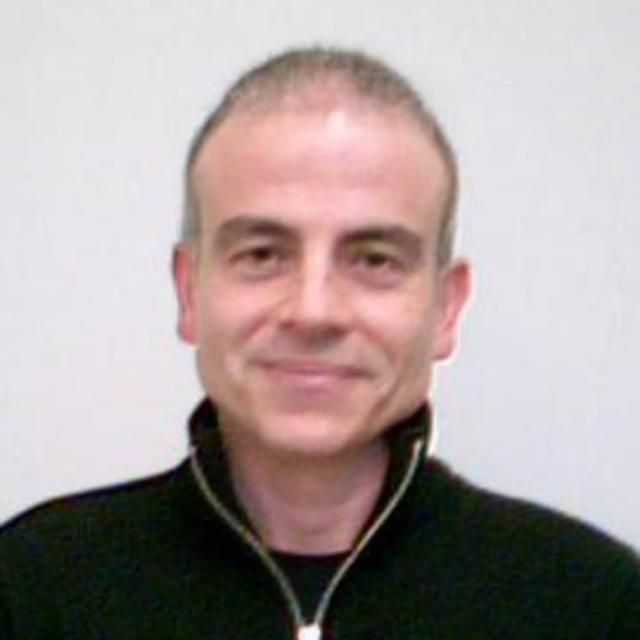
\includegraphics[width=0.5\linewidth]{./laudelino}\\           
            \textbf{Laudelino Cordeiro Bastos}\\
            
\includegraphics[width=0.3\linewidth]{qrcode-laudelino}           
            %Department of Subject\\
            %University Name
        \end{column}
        
        % Column 2: Profile Picture
        \begin{column}{0.5\textwidth}
            \centering
            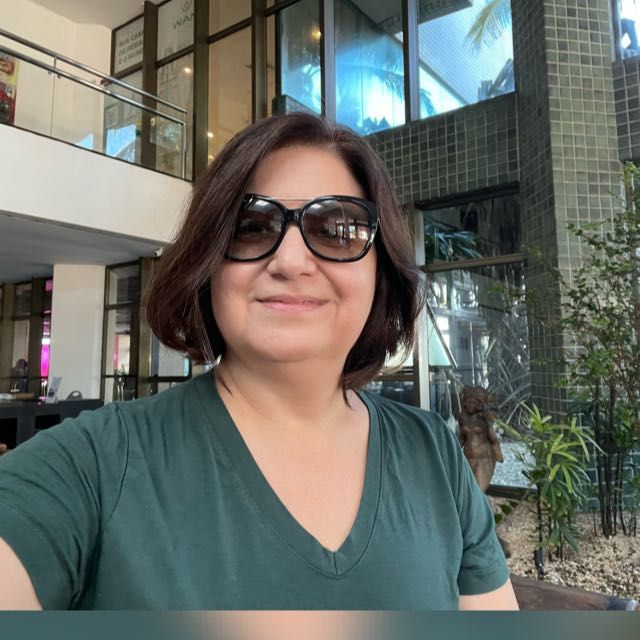
\includegraphics[width=0.5\linewidth]{./emer} \\          
            \textbf{Maria Claudia Figueireido Pereira Emer}\\
            
\includegraphics[width=0.3\linewidth]{qrcode-emer}           
        \end{column}
    \end{columns}
\end{frame}
\begin{frame}{Agradecimentos}
\begin{columns}
        % Column 1: Name
        \begin{column}{0.5\textwidth}
            \centering
            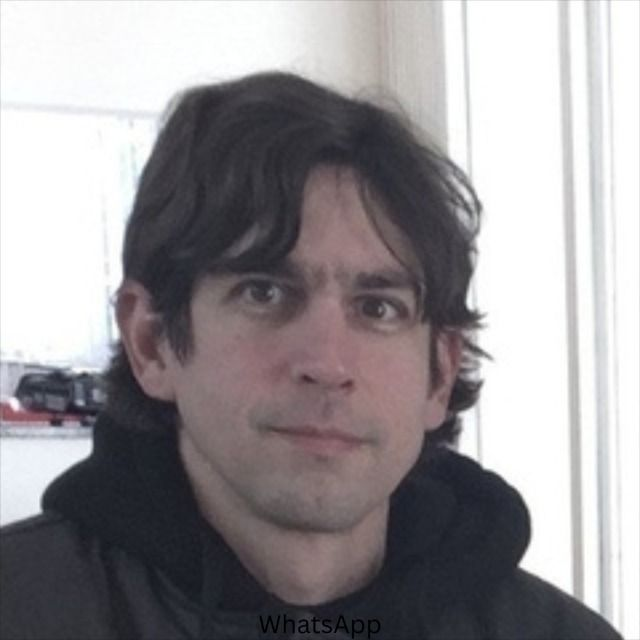
\includegraphics[width=0.6\linewidth]{./adolfo}\\           
            \textbf{Adolfo Gustavo Serra Seca Neto}\\
        \end{column}

        \begin{column}{0.4\textwidth}
            \centering
            
\includegraphics[width=0.5\linewidth]{qrcode-adolfo}           
        \end{column}
        
    \end{columns}
\end{frame}
\section{Introdução}

\begin{frame}{Práxis}
\large
O ensino de programação é uma atividade multidisciplinar que demanda uma práxis
pedagógica apurada – ou seja, uma constante reflexão que integre teoria e prática em sala de aula. Uma estratégia comum é utilizar exemplos do cotidiano para estimular a resolução de problemas por meio de algoritmos. Contudo, avaliar a qualidade desses algoritmos exige ir além da verificação funcional.

\end{frame}

\begin{frame}{Dificuldades no aprendizado}
\large 
Ainda segundo (Raabe; Silva, 2005), as dificuldades no aprendizado de programação
podem ser categorizadas em três grupos distintos, que vão além da simples aptidão individual:
Problemas de natureza didática (relacionados aos métodos de ensino), cognitiva (relacionados
aos desafios de raciocínio lógico e abstração) e afetiva(relacionados à motivação, ansiedade
e confiança do aluno). Essa categorização sistêmica ajuda a entender que o desafio requer
iniciativas diferentes.

\end{frame}
\begin{frame}{Diagrama de Venn: Integração de Disciplinas}
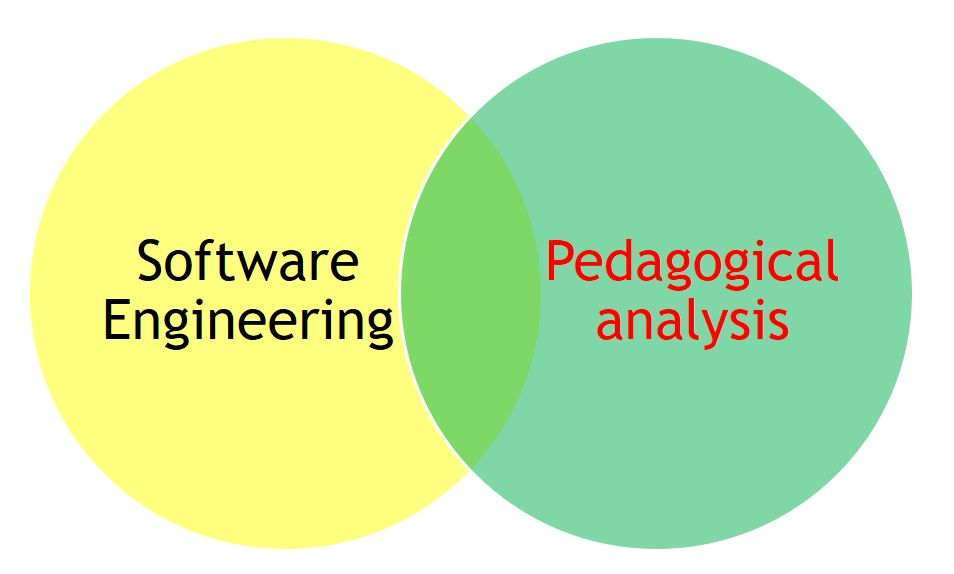
\includegraphics[scale=0.35]{venn}
\end{frame}

\begin{frame}{Logging: Conceitos e aplicações na Engenharia de Software}
As práticas de registro de rastros em sistemas computacionais abrangem diversos conceitos. Como exemplo, a taxonomia de (\textit{Gu et al., 2022}) define os seguintes elementos fundamentais: \\
\vspace{0.2in}
\begingroup
\renewcommand{\arraystretch}{1.2}
\begin{tabular}{p{0.3\textwidth}p{0.3\textwidth}p{0.3\textwidth}}
    • Log statement       & • Log message     & • Log \\
    • Log level           & • Log content     & • Log location \\
    • Log placement       & • Logging         & • Logging practice \\
\end{tabular}
\endgroup

\end{frame}
\large
\begin{frame}{A importância dos logs}
Segundo (Rice; Borgman, 1983), o monitoramento de sistemas pode ser entendido como
um registro automático de transações. A importância dos \textit{logs} é vasta, sendo utilizados em tarefas como detecção de anomalias, depuração, diagnóstico de desempenho e modelagem de comportamento de sistemas (Fu et al., 2014). Estudos como o de (Yang \textit{et al}., 2021) confirmam que os desenvolvedores os utilizam primariamente para análise de problemas, buscando informações como a propagação de erros, \textit{timestamps} e o \textit{dataflow} entre componentes.

\end{frame}

\begin{frame}{Análise de logs como Ferramenta Educacional}
\begin{table}[h]
\centering
\normalsize
\caption{Comparação entre abordagens de avaliação em programação}
\label{tab:comparacao-avaliacao}
\begin{tabular}{p{0.5\textwidth}p{0.5\textwidth}}
\hline
\textbf{Avaliação Tradicional} & \textbf{Avaliação com Análise de \textit{Logs}} \\
\hline
Foca no produto final (código) & Foca no processo de desenvolvimento \\
Analisa o que foi produzido & Analisa como foi produzido \\
Avaliação predominantemente quantitativa & Inclui dimensões qualitativas do aprendizado \\
Visão estática do conhecimento & Visão dinâmica da curva de aprendizagem \\
Foco no indivíduo & Permite análise individual e em grupo \\
\hline
\end{tabular}
\end{table}
\end{frame}
%\subsection{Contextualização}
%\begin{frame}{Contextualização}
%
%    \begin{itemize}
%        \item Item 1
%        \item Item 2
%        \item Item 3
%    \end{itemize}
%
%\end{frame}
%
%\begin{frame}{Motivação}
%
%    Texto com a motivação do trabalho.
%
%\end{frame}
%
%\begin{frame}{Justificativa}
%
%    Texto com a justificativa do trabalho.
%
%\end{frame}

\subsection{Objetivos}
\begin{frame}{Objetivo geral}
\large
    O objetivo deste trabalho é desenvolver e implementar um plugin para coleta e análise de logs durante o processo de ensino-aprendizagem de programação, com o intuito de fornecer métricas que auxiliem na identificação de dificuldades dos alunos, na personalização do ensino e no aprimoramento das práticas pedagógicas

\end{frame}

\subsection{Objetivos}
\begin{frame}{Objetivos específicos}

    \begin{enumerate}
	\item \textbf{O que pretende:} Investigar o processo de aprendizagem de programação por meio da análise de logs acadêmicos, identificando padrões e dificuldades comuns entre os estudantes.
	\item \textbf{Como pretende:} Utilizando ferramentas de captura de eventos durante as aulas de programação, processando os dados coletados e organizando-os em um repositório acessível.
	\item \textbf{Por que pretende:} Para melhorar o ensino de programação, oferecendo outras características, objetos de estudos baseados em dados quantitativos e criando um recurso (\textit{dataset}) que possa ser utilizado por outros pesquisadores e educadores.
\end{enumerate}
\end{frame}

\begin{frame}{Tarefas metodológicas}
\begin{enumerate}
	\item Desenvolver um \textit{plugin} para registro de eventos durante as aulas de programação.
	\item Implementar o \textit{plugin} na IDE utilizada na disciplina, com a anuência da instituição e dos estudantes.
	\item Coletar, sincronizar e armazenar dados de eventos gerados durante o experimento.
	\item Desenvolver um \textit{dataset} com os dados coletados, organizados por turma, instituição e disciplina.
\end{enumerate}

\end{frame}
\begin{frame}{Contribuições esperadas}
\begin{enumerate}
    \item Um Mapeamento Sistemático da Literatura sobre uso de logs no ensino de programação focado 
    principalmente nas instituições de ensino brasileiras. 
     \item Desenvolvimento de um plugin para uma IDE que possa auxiliar na coleta de logs durante o uso do 
     programa e desenvolvimento de códigos.
     \item Desenvolvimento e disponibilidade de um \textit{dataset} dos logs gerados de forma aberta, respeitando a 
     privacidade e dados sigilosos de todos os participantes. 
\end{enumerate}

\end{frame}
%%%%%%%%%%%%%%%%%%%%%%%%%%%%%%%%%%%%%%%%%%%%%%%%%%%%%%%%%%%%%

\section{Metodologia}

\begin{frame}{Métodos de desenvolvimento}
\begin{itemize}
\item Revisão Sistemática da Literatura
\item Survey Exploratório
\item Design Science Research
\end{itemize}
\end{frame}

%%%%%%%%%%%%%%%%%%%%%%%%%%%%%%%%%%%%%%%%%%%%%%%%%%%%%%%%%%%
\section{Revisão Sistemática da Literatura}
\begin{frame}{Lista de repositórios}
\centering
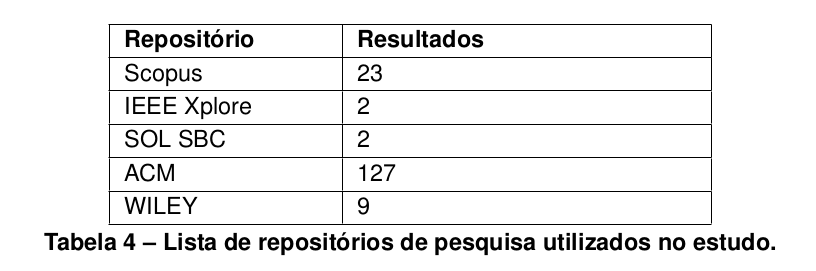
\includegraphics[scale=.4]{table4}
\end{frame}

\begin{frame}{Palavras-chave e Operadores}
\centering
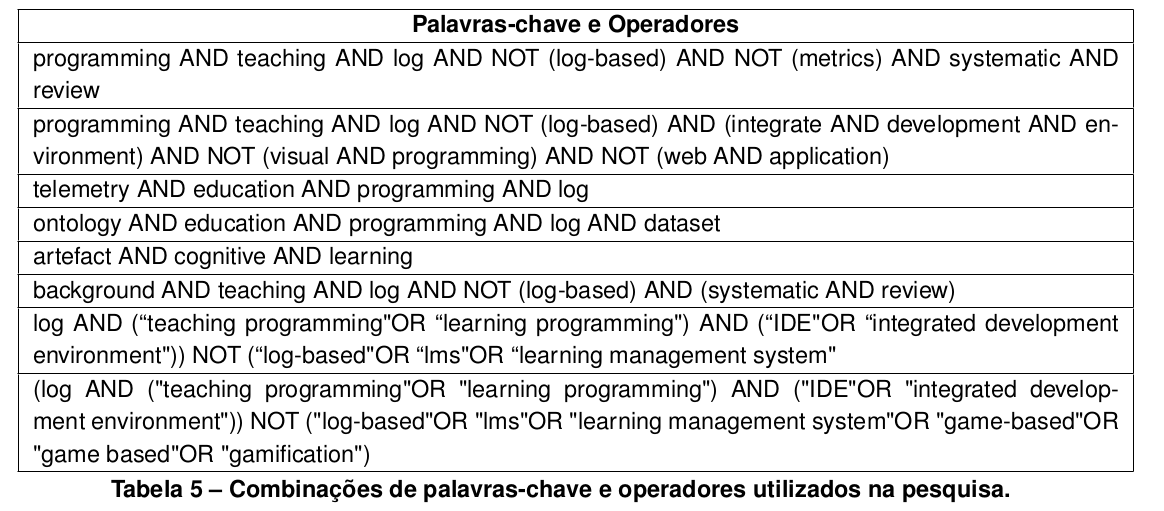
\includegraphics[scale=.28]{table5}
\end{frame}

\begin{frame}{Critério de Inclusão}
\begin{enumerate}
\item Relevância temática
\item Revisão sistemática
\end{enumerate}
\end{frame}

\begin{frame}{Critério de Exclusão}
\begin{enumerate}
\item Log-based
\item Uso de logs em outras áreas da educação
\item Learning Management System(LMS)
\item Game-based learning
\end{enumerate}
\end{frame}

\begin{frame}{Resultados da busca e caracterização dos Estudos}
\begin{figure}
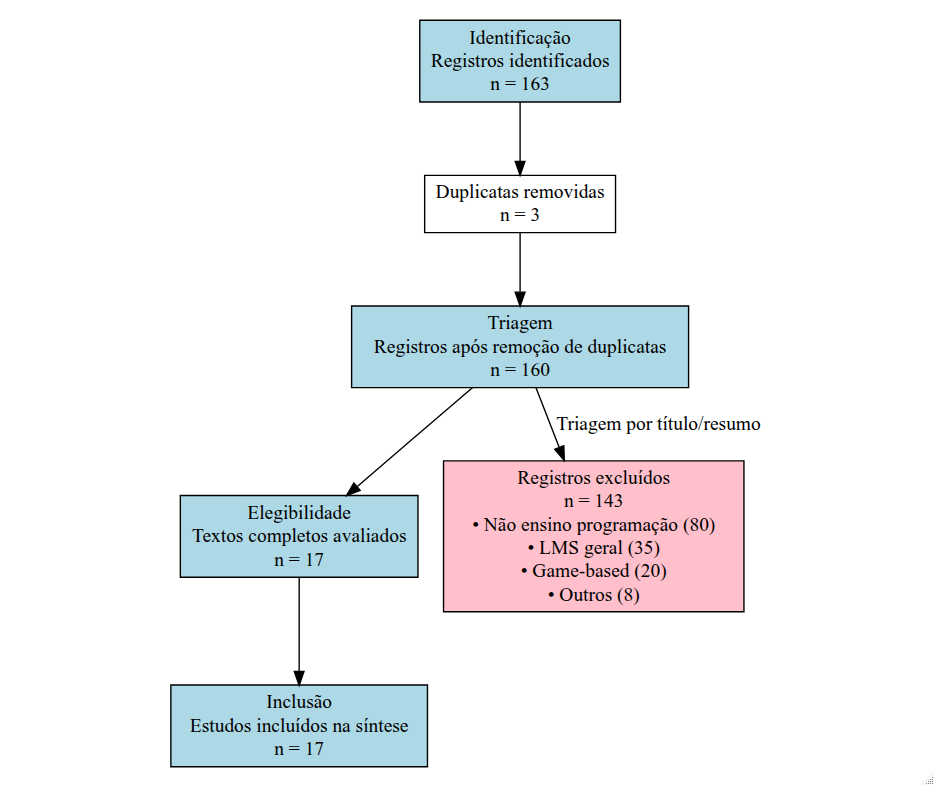
\includegraphics[scale=0.22]{prisma}
\caption{Fluxograma PRISMA do processo de seleção de estudos}
\end{figure}
\end{frame}

\begin{frame}{Características dos 17 estudos incluídos na síntese qualitativa} 
\centering
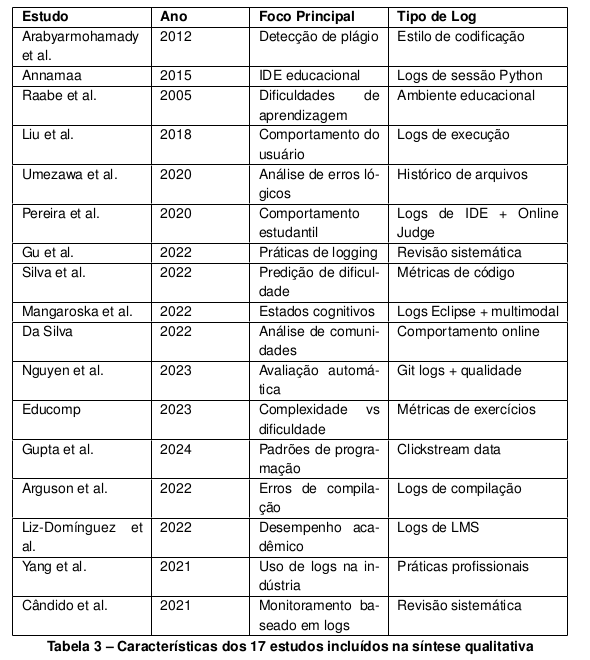
\includegraphics[scale=.3]{table3}
\end{frame}


%%%%%%%%%%%%%%%%%%%%%%%%%%%%%%%%%%%%%%%%%%%%%%%%%%%%%%%%%%%%%

\begin{frame}{Questões de Pesquisas}
\begin{enumerate}
\item QP1 - Quais são os principais objetivos e aplicações do uso de logs no ensino de programação?
\item QP2 - Quais ferramentas, métodos e métricas são mais utilizados para capturar, armazenar e analisar logs em ambientes de ensino de programação?
\end{enumerate}
\end{frame}
\section{Questão de Pesquisa 1}
\begin{frame}{Objetivos categorizados em quatro áreas principais}
Os objetivos identificados foram categorizados em quatro áreas principais:
\vspace{0.3in}
\begin{itemize}
    \item \textbf{Detecção de Dificuldades} (6 estudos): Umezawa (2020), Pereira (2020), Silva (2022), Educomp (2023), Arguson (2022), Raabe (2005)
    \item \textbf{Análise de Comportamento} (5 estudos): Gupta (2024), Liu (2018), Mangaroska (2022), Da Silva (2022), Liz-Domínguez (2022)
    \item \textbf{Qualidade de Código} (3 estudos): Arabyarmohamady (2012), Nguyen (2023), Annamaa (2015)
    \item \textbf{Práticas e Ferramentas} (3 estudos): Gu (2022), Yang (2021), Cândido (2021)
\end{itemize}
\end{frame}

\begin{frame}{3W1H}

De acordo com (Gu \textit{et al.}, 2022) ``A obtenção de logs é um processo que deve ser guiado por quatro questões fundamentais, conhecidas como 3W1H:
\vspace{0.3in}
\begin{itemize}
    \item Why (Por quê): Qual é o objetivo da coleta de logs?
    \item Where (Onde): Em quais partes do sistema ou código os logs devem ser coletados?
    \item What (O que): Quais informações ou eventos devem ser registrados nos logs?
    \item How (Como): De que forma os logs serão coletados, armazenados e analisados?
\end{itemize}
\end{frame}
\section{Questão de Pesquisa 2}
\begin{frame}{Ferramentas, métodos e métricas}
\begin{itemize}
\item CodeBench (Pereira \textit{et al.,} 2020)
\item Alignment-based matching (Lit \textit{et al.,}2018)
\item Plugin para Eclipse que possui uma aba - (Mangaroska \textit{et al.,} 2022)
\item Thonny (Annamaa, 2015)
\item ProgEdu (Nguyen; Ha; Chen, 2023)
\end{itemize}
\end{frame}
\section{Survey Exploratório}
\begin{frame}{Survey}
\vspace{0.3in}
Para entender o uso de logs no ensino de programação, buscamos informações de ou-
tras instituições de ensino. Para ter informações sobre como alguns nós da Rede EPTC tratam o assunto, foi elaborado um questionário. A partir das respostas, os dados foram tabulados e gráficos foram gerados a partir dessas informações.
\vspace{0.33in}
\begin{figure}[!ht]

\includegraphics[scale=0.2]{qrcode-survey}
\caption{Link para o Google Forms}
\end{figure}
\end{frame}
\begin{frame}{Instrumento de pesquisa}
\begin{enumerate}
    \item[2.] Você usa alguma ferramenta de log no apoio ao ensino de programação? \\ (~~) Sim (~~) Não
    \item[3.] O uso de ferramentas de logs pode auxiliar no monitoramento e compreensão no empenho dos estudantes?  \\
    (1) Discordo Totalmente (2) Discordo Parcialmente (3) Neutro (4) Concordo Parcialmente (5) Concordo Totalmente
    \item[4.] O uso de ferramentas de logs pode ajudar a tomar decisões para melhorar o rendimento e evitar a desistência de uma disciplina? \\
    (1) Discordo Totalmente (2) Discordo Parcialmente (3) Neutro (4) Concordo Parcialmente (5) Concordo Totalmente
    \item[5.] O uso de ferramentas de logs pode auxiliar no ensino de programação? \\
    (1) Discordo Totalmente (2) Discordo Parcialmente (3) Neutro (4) Concordo Parcialmente (5) Concordo Totalmente
    \end{enumerate}
 \end{frame}
 \begin{frame}{Continua}
 \begin{enumerate}
     \item[6.] Um dataset pode ser criado e estudado a partir de logs no ensino da programação? \\
    (1) Discordo Totalmente (2) Discordo Parcialmente (3) Neutro (4) Concordo Parcialmente (5) Concordo Totalmente
    \item[7.] Sobre usar ferramentas de correções de códigos mais automatizado possível nas aulas de ensino de programação. O que pensa a respeito sobre o uso? \\
    (1) Discordo Totalmente (2) Discordo Parcialmente (3) Neutro (4) Concordo Parcialmente (5) Concordo Totalmente
    \item[8.] Plugins podem auxiliar na criação/ensino  de algoritmos? \\
    (1) Discordo Totalmente (2) Discordo Parcialmente (3) Neutro (4) Concordo Parcialmente (5) Concordo Totalmente
    \item[9.] Qual IDE é utlizado nas aulas? \\ (~~)Visual Studio (~~) Intellij IDEA (~~) Eclipse ( ) Outro - Descrever
    \item[10.] Ferramenta de análise de algoritmos \\ (~~)Code Bench (~~) Juiz Online (~~) LAPLE (~~) Outro: Descrever
    \item[11.] Se tiver disponível um plugin de log para o apoio ao ensino de programação, você usaria? \\ (~~) Sim (~~) Não
\end{enumerate}

\end{frame}
\begin{frame}{Questões 2 e 3}
\begin{figure}
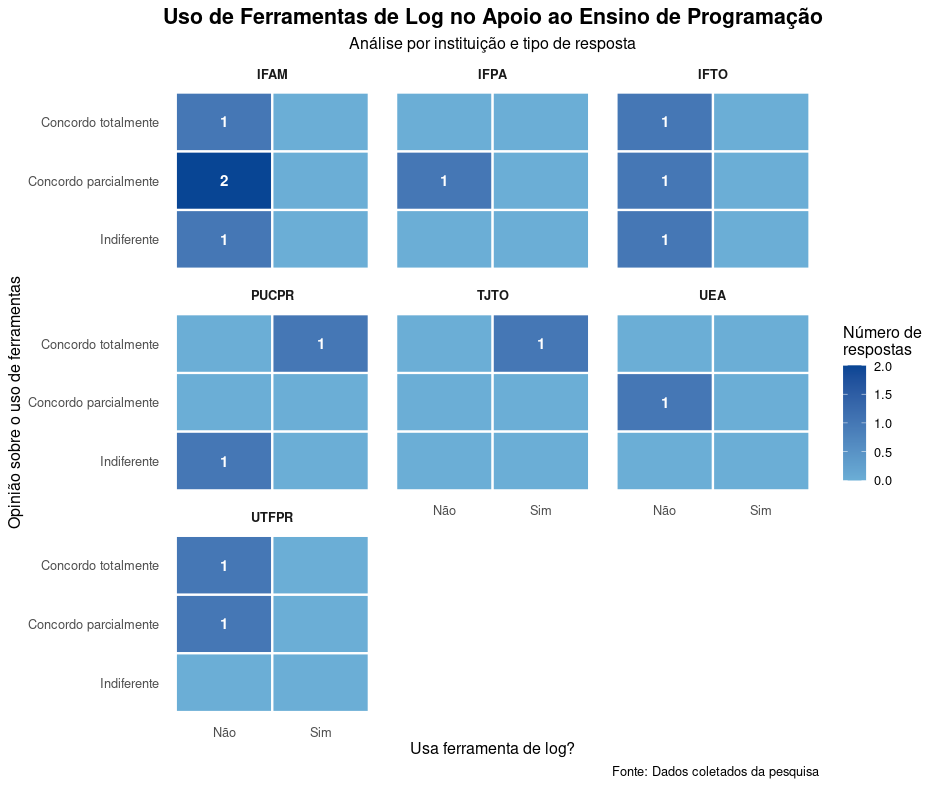
\includegraphics[scale=0.26]{questao2}
%\caption{Mapa de calor representando a frequência de uso e familiaridade com diferentes ferramentas tecnológicas (Perguntas 2 e 3). As cores mais quentes indicam maior frequência de uso ou familiaridade, permitindo identificar quais ferramentas são mais dominadas pelos participantes da pesquisa.}
\end{figure}
\end{frame}
\begin{frame}{Questões 4 e 5}
\centering
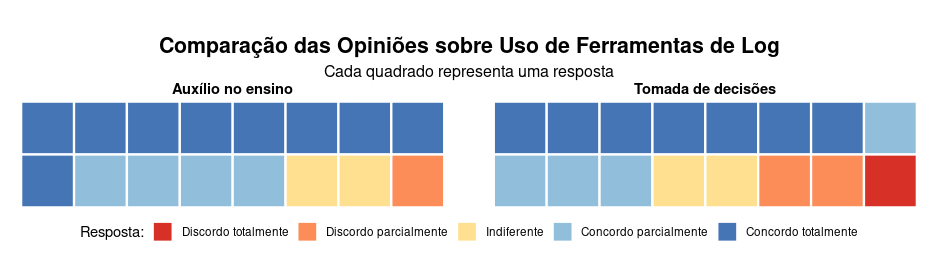
\includegraphics[scale=0.45]{questao34}
\end{frame}
\begin{frame}{Questões 6 e 7}
\centering
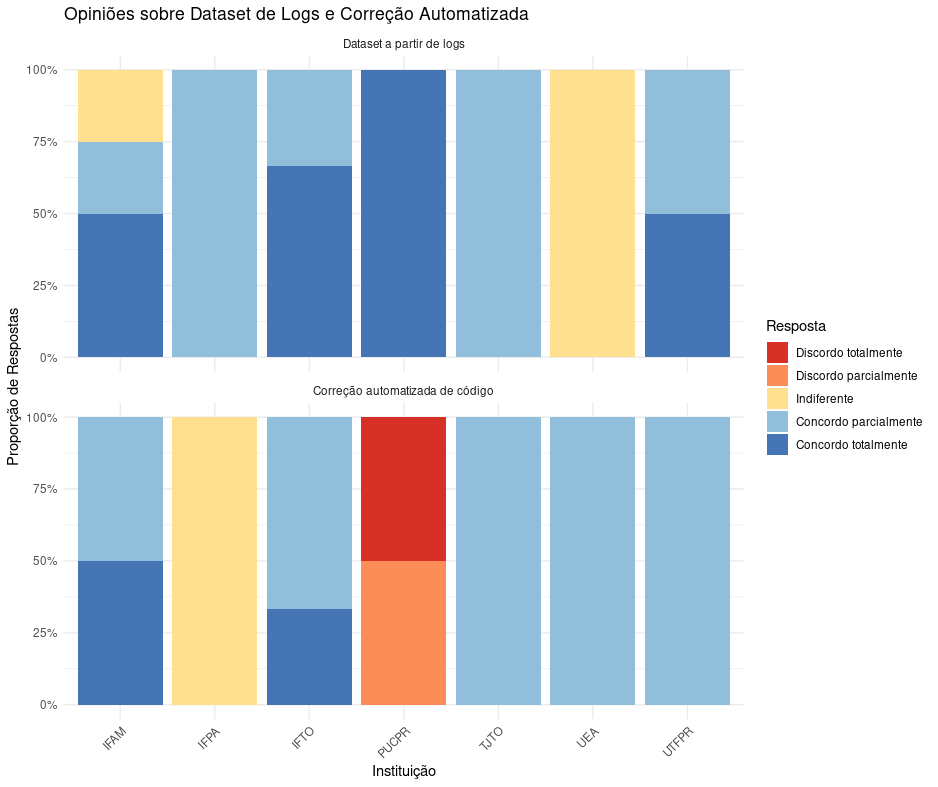
\includegraphics[scale=0.23]{questao56}
\end{frame}
\begin{frame}{Questões 9 e 11}
\centering
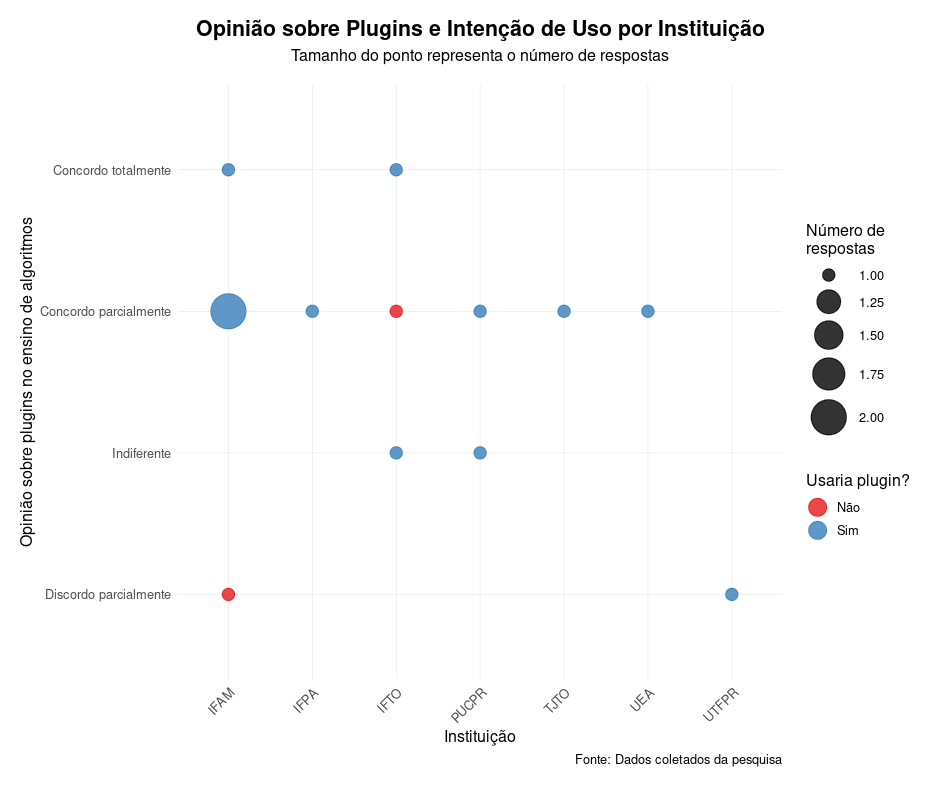
\includegraphics[scale=0.25]{questao911}
\end{frame}
\begin{frame}{Questões 5 e 6}
\centering
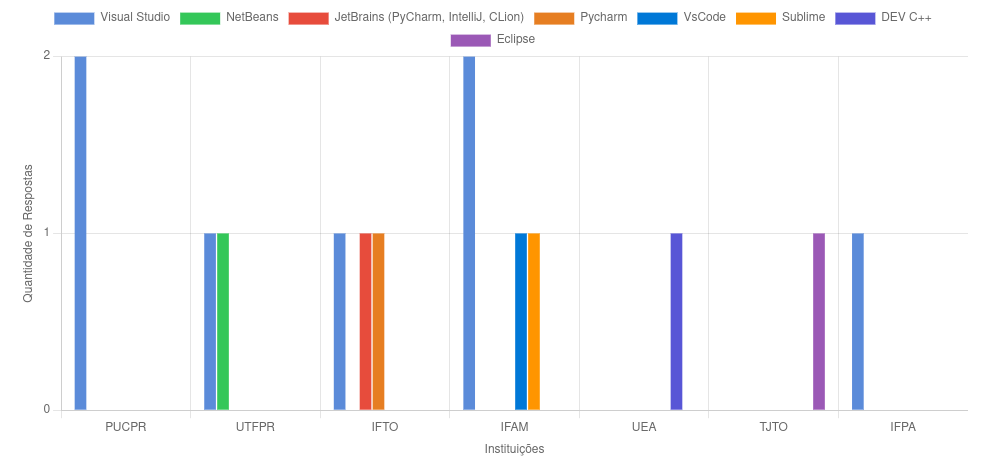
\includegraphics[scale=0.43]{ide}
\end{frame}

\section{Design Science Research}
\begin{frame}{Design Science Research}
Este trabalho adota a abordagem de Design Science Research (DSR), conforme proposto por (\textit{Peffers et al., 2007}) e (\textit{Hevner et al., 2004}). O DSR é adequado para pesquisas que visam desenvolver e avaliar artefatos que resolvam problemas identificados em contextos organizacionais e educacionais.
\vspace{0.35in}

O processo de DSR será executado em quatro atividades principais:

\begin{enumerate}
\item Identificação do Problema e motivação
\item Definição dos Objetivos da solução
\item Design e Desenvolvimento
\item Especificação de Requisitos do Artefato
\end{enumerate}
\end{frame}

\begin{frame}{Identificação do Problema e Motivação}
\large
O problema central identificado é a carência de ferramentas específicas para captura e análise de logs acadêmicos no ensino de programação, especialmente no contexto da região Amazônica. Esta lacuna limita a capacidade de docentes e instituições em identificar dificuldades de aprendizagem de forma objetiva e baseada em dados.
\end{frame}
\begin{frame}{Definição dos Objetivos da Solução}
Com base no problema identificado, definiram-se os seguintes objetivos:\\
\vspace{0.3in}
\textbf{Objetivo Geral:}
Desenvolver e validar um \textit{plugin} para coleta e análise de logs durante o processo de ensino-aprendizagem de programação.
\vspace{0.3in}\\
\textbf{Objetivos Específicos:}
\begin{enumerate}
    \item Desenvolver um \textit{plugin} para registro de eventos em IDE
    \item Implementar o plugin na IDE utilizada na disciplina
    \item Coletar, sincronizar e armazenar dados de eventos
    \item Desenvolver um dataset com os dados coletados
    \item Validar a abordagem por meio de experimentos controlados
\end{enumerate}

\end{frame}
\begin{frame}{Design e Desenvolvimento}
O design e desenvolvimento segue uma abordagem iterativa, pois os dados serão coletados quando os estudantes desenvolvem as atividades envolvendo algoritmos. A arquitetura do artefato compreendendo quatro módulos principais:\\
\vspace{0.3in}

\begin{itemize}
\item Módulo de captura: Implementa a coleta de palavras reservadas e o carimbo temporal (\textit{timestamp})
\item Módulo de serialização: Transforma os eventos em uma estrutura JSON
\item Módulo de armazenamento: Gerencia os arquivos localmente
\item Módulo de configuração: Confirma se a extensão está funcionando corretamente e coletando os logs
\end{itemize}
\end{frame}
\begin{frame}{Especificação de requisito do artefato}
Para garantir que o \textit{plugin} \textit{Logado} atenda aos objetivos da pesquisa e às necessidades dos usuários finais, foi realizada uma etapa de especificação de requisitos. A análise inicial identificou dois atores principais, cujas necessidades são sumarizadas na Tabela \ref{tab:analise-atores}.

\begin{table}[h!]
\centering
\caption{Análise de atores e necessidades do sistema}
\label{tab:analise-atores}
\begin{tabular}{|p{0.3\linewidth}|p{0.3\linewidth}|p{0.3\linewidth}|}
\hline
\textbf{Ação} & \textbf{Discente} & \textbf{Pesquisador} \\
\hline
Funções necessárias & Enviar dados de execução & Desenvolver/testar plugin \\
\hline
Necessidade principal & Instalar e usar o plugin & Validar processamento de logs \\
\hline
Operações CRUD & Enviar (criar) logs & Gerenciar usuários e dataset \\
\hline
\end{tabular}
\end{table}
\end{frame}
\begin{frame}{Caso de uso: Discentes}
\begin{figure}
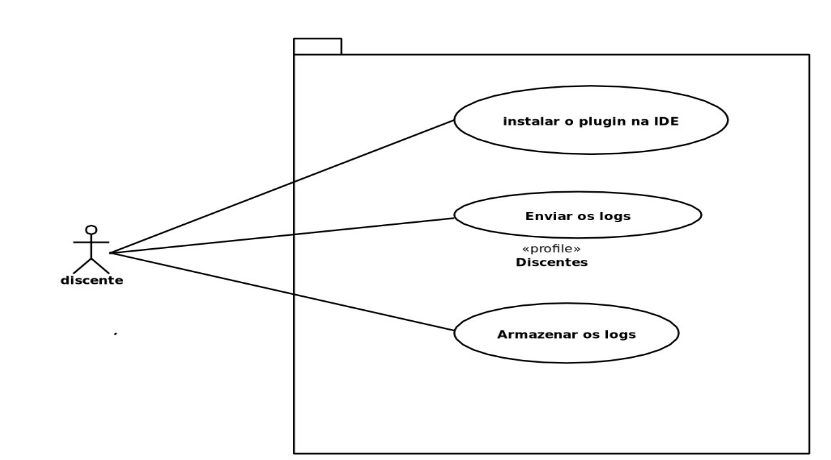
\includegraphics[scale=0.35]{discente}
\caption{Visão do Estudante}
\end{figure}
\end{frame}
\begin{frame}{Caso de uso: Pesquisa}
\begin{figure}
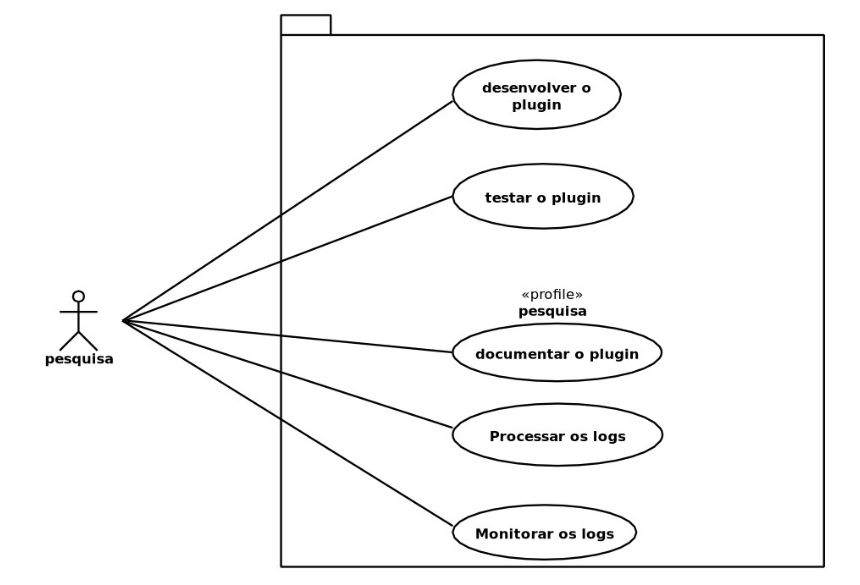
\includegraphics[scale=0.3]{pesquisa}
\caption{Visão da Pesquisa}
\end{figure}
\end{frame}

\begin{frame}{Requisitos Funcionais - Discente}
Os requisitos funcionais definem as funcionalidades que o sistema deve executar.\\ \vspace{0.1in} Para o ator \textbf{Discente}, um \textit{plugin} deve:
\begin{itemize}
    \item \textbf{RF01:} Registrar automaticamente eventos de edição de código (e.g., inserção, deleção de caracteres).
    \item \textbf{RF02:} Capturar eventos de compilação e execução de código, incluindo sucesso ou falha.
    \item \textbf{RF03:} Armazenar localmente os logs com \textit{timestamp} preciso.
    \item \textbf{RF04:} Transmitir os logs anonimizados para um servidor remoto de forma assíncrona.
    \item \textbf{RF05:} Exibir notificações de confirmação de operações para o usuário.
\end{itemize}

Para o ator \textbf{Pesquisador}, um \textit{plugin} deve:
\begin{itemize}
    \item \textbf{RF06:} Fornecer uma interface de configuração para parametrizar os eventos a serem capturados.
    \item \textbf{RF07:} Gerar identificadores únicos anônimos para cada sessão de uso.
\end{itemize}
\end{frame}

\begin{frame}{Requisitos Não-funcionais}
Estes requisitos definem os critérios de qualidade para o sistema: \\ \vspace{0.3in}
\begin{itemize}
    \item \textbf{RNF01 (Desempenho):} um \textit{plugin} não deve impactar significativamente o desempenho da IDE. O tempo de resposta deve ser inferior a 100ms para operações de registro.
    \item \textbf{RNF02 (Usabilidade):} A instalação e o uso devem ser simples, não requerendo configuração complexa por parte do discente.
    \item \textbf{RNF03 (Confiabilidade):} um \textit{plugin} deve garantir a persistência dos logs mesmo em caso de fechamento inesperado da IDE.
    \item \textbf{RNF04 (Segurança e Privacidade):} Todos os dados pessoais devem ser anonimizados antes do envio ao servidor, conforme a LGPD.
\end{itemize}
\end{frame}
\begin{frame}{Desenvolvimento do Artefado}
\begin{center}
\textsl{LOGADO - Logs Acadêmico }
\end{center}
\vspace{0.5in}
   \begin{columns}[T]
        \begin{column}{0.5\textwidth}
            \centering
            
\includegraphics[scale=0.25]{vscode}\\
            \textbf{Visual Studio Code}
            
           \end{column}
        
        \begin{column}{0.5\textwidth}
            \centering
            
\includegraphics[scale=0.15]{logado}\\
            \textbf{Logado}
        \end{column} 
    \end{columns}

\end{frame}
\begin{frame}{VSCE}
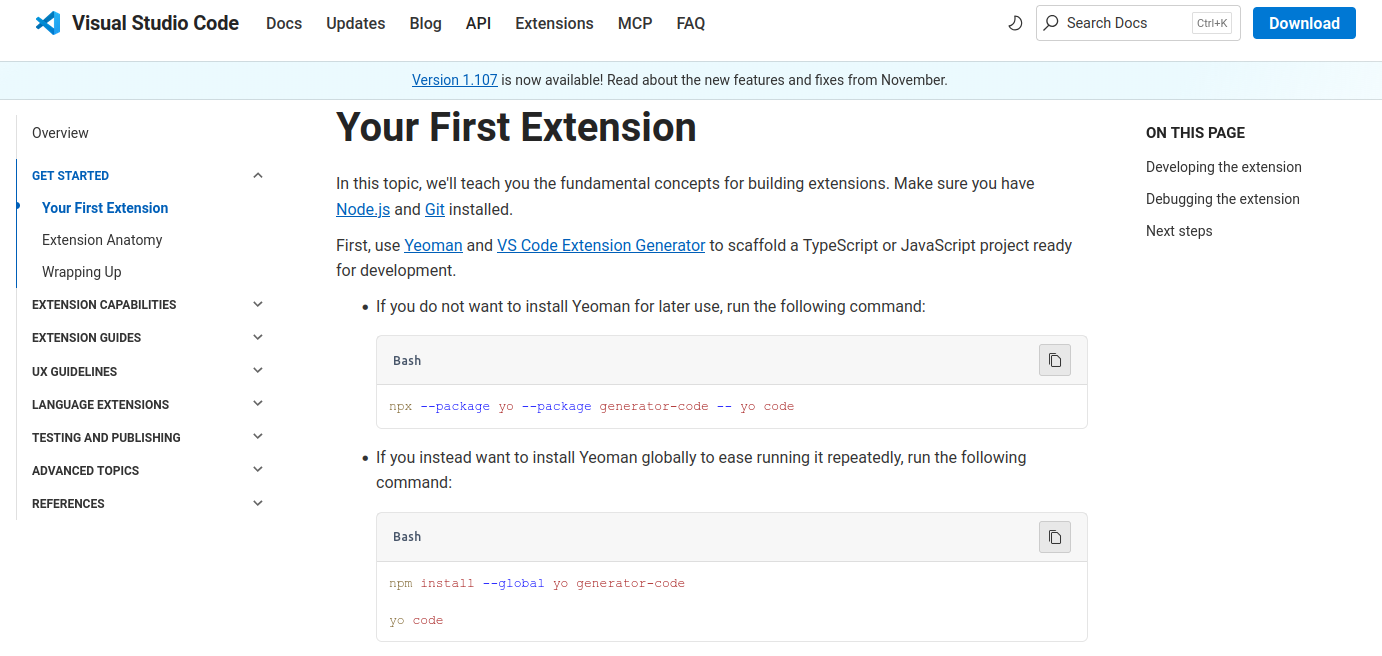
\includegraphics[scale=0.3]{vsce}
\end{frame}
\begin{frame}{yo-code}
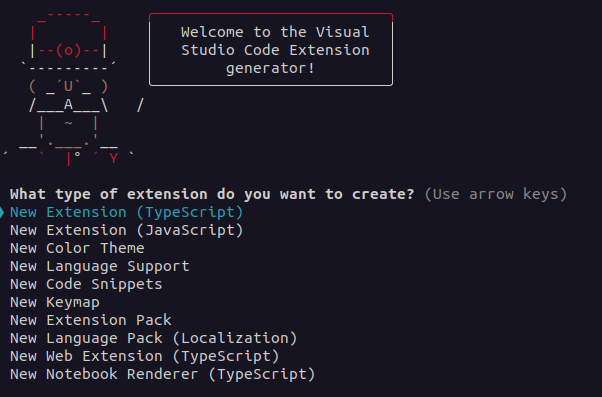
\includegraphics[scale=0.45]{yocode}
\end{frame}
\begin{frame}{LOGADO}
\begin{itemize}
\item Palavras reservadas (linguagem de programação)
\item Carimbos temporais (timestamps)
\item Salvar os logs (e armazenar, sincronizar, agrupar)
\end{itemize}
\end{frame}
\begin{frame}{Palavras reservadas}
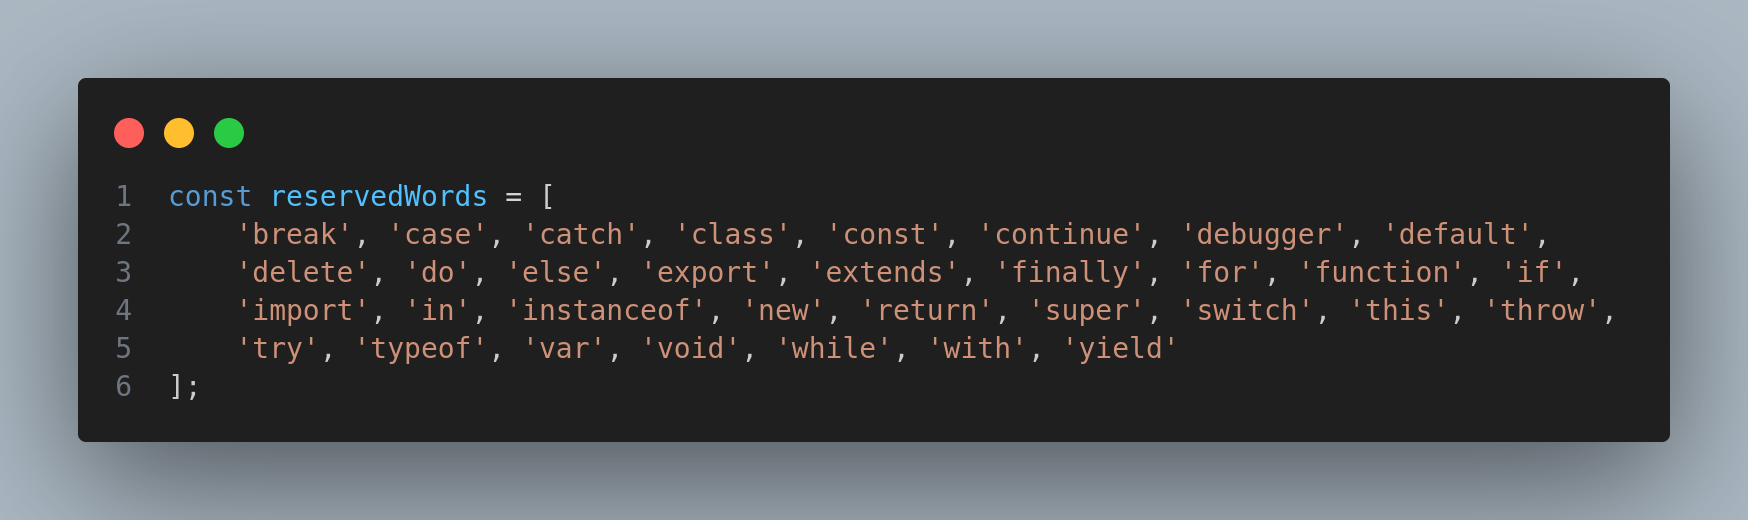
\includegraphics[scale=0.22]{keywords}
\end{frame}
\begin{frame}{Carimbo temporal}
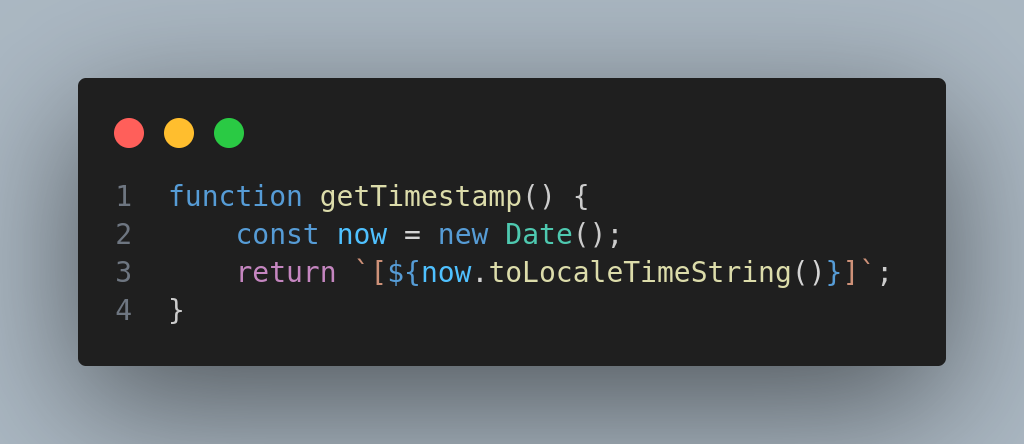
\includegraphics[scale=0.34]{timestamp}
\end{frame}


\section{Cronograma}
\begin{frame}{Cronograma}
\begin{center}
\begin{figure}
	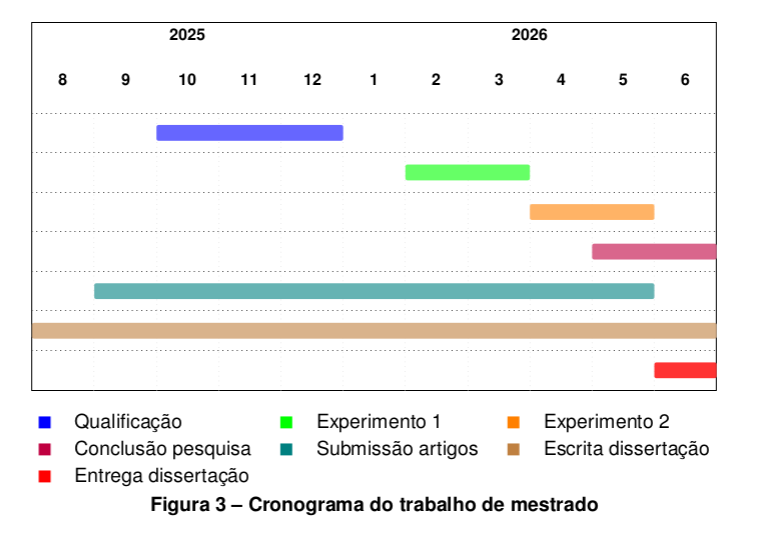
\includegraphics[scale=0.3]{cronograma}
\end{figure}
\end{center}
\end{frame}
\section{Artigo - Evento}
\begin{frame}{LACLO}
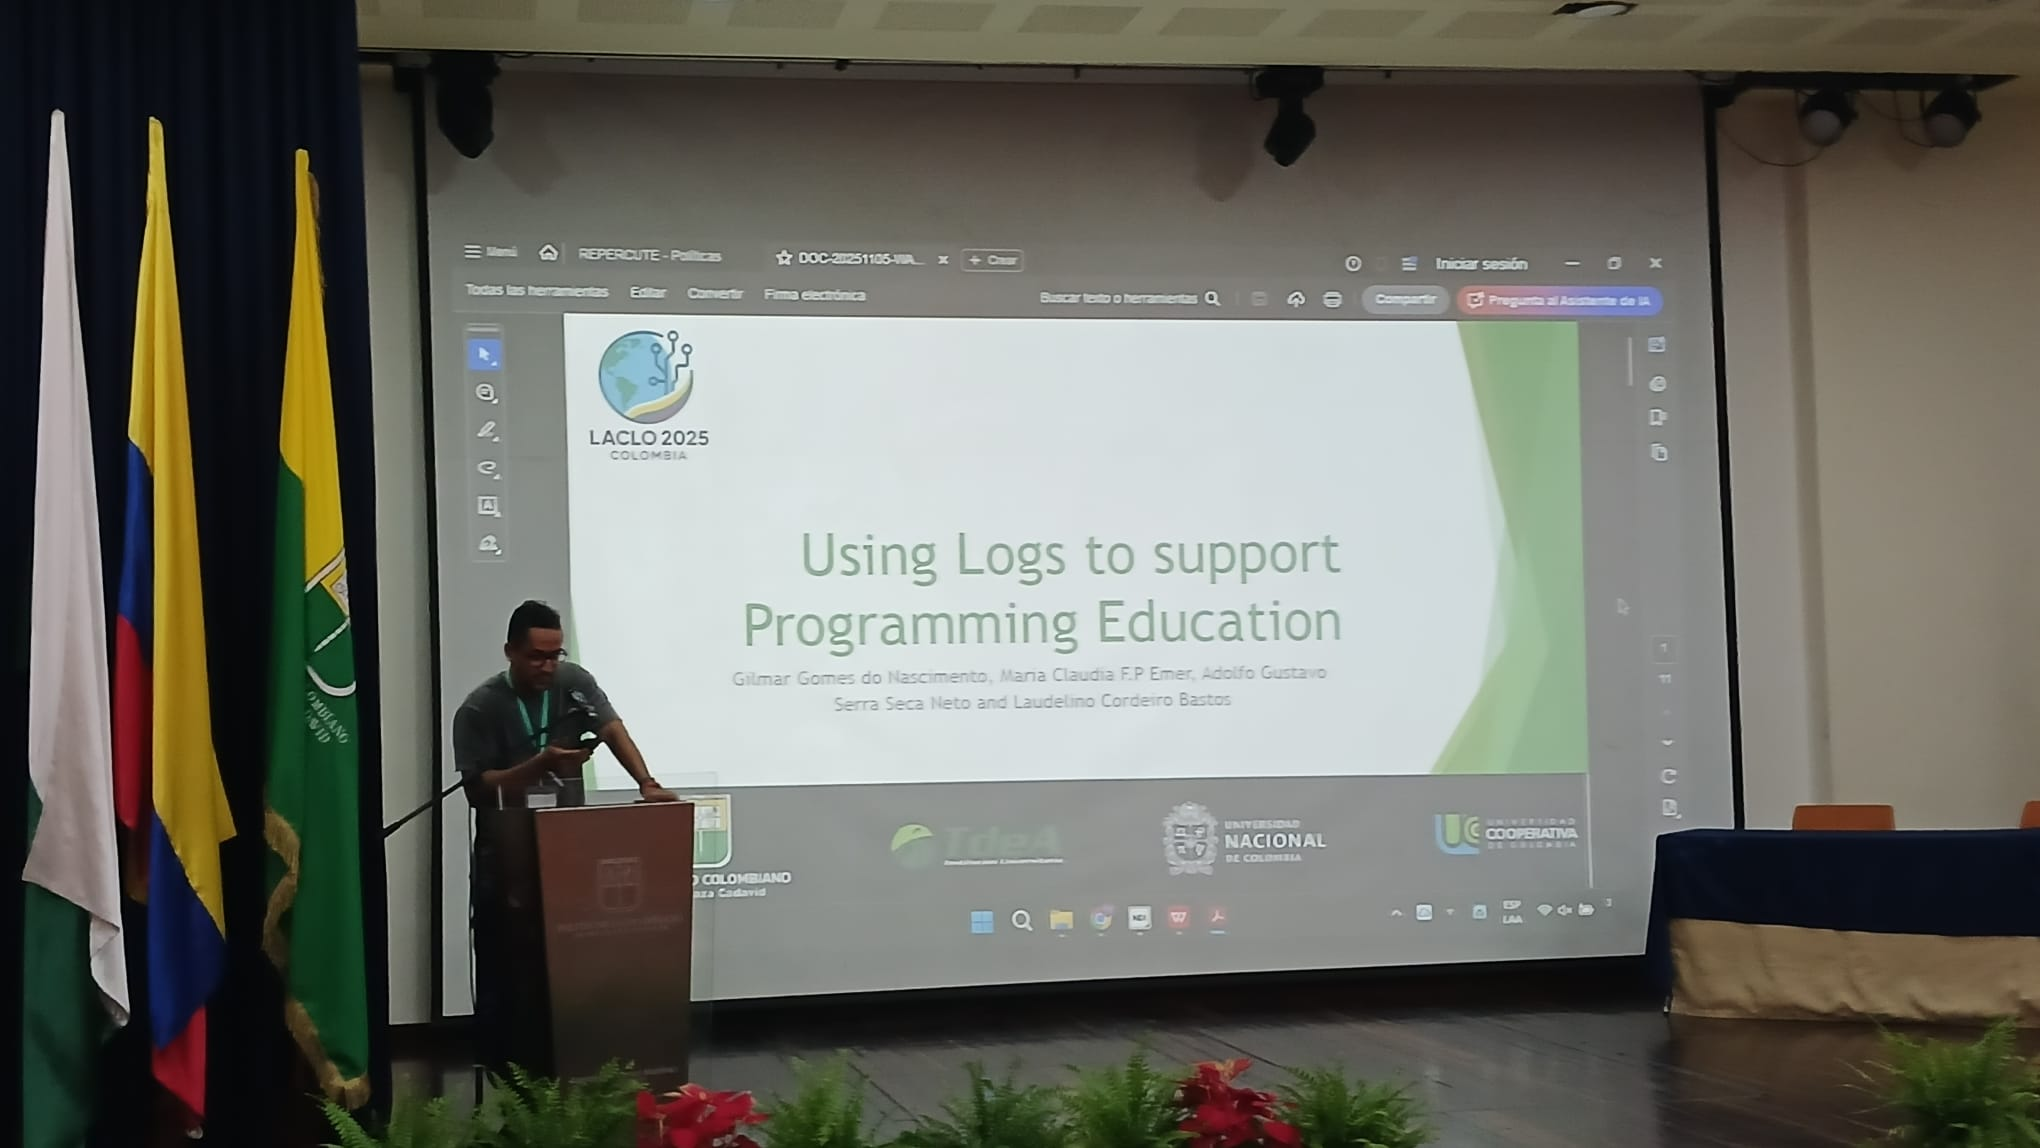
\includegraphics[scale=0.2]{laclo}

\end{frame}
\section{Referências}
\begin{frame}{Referências}
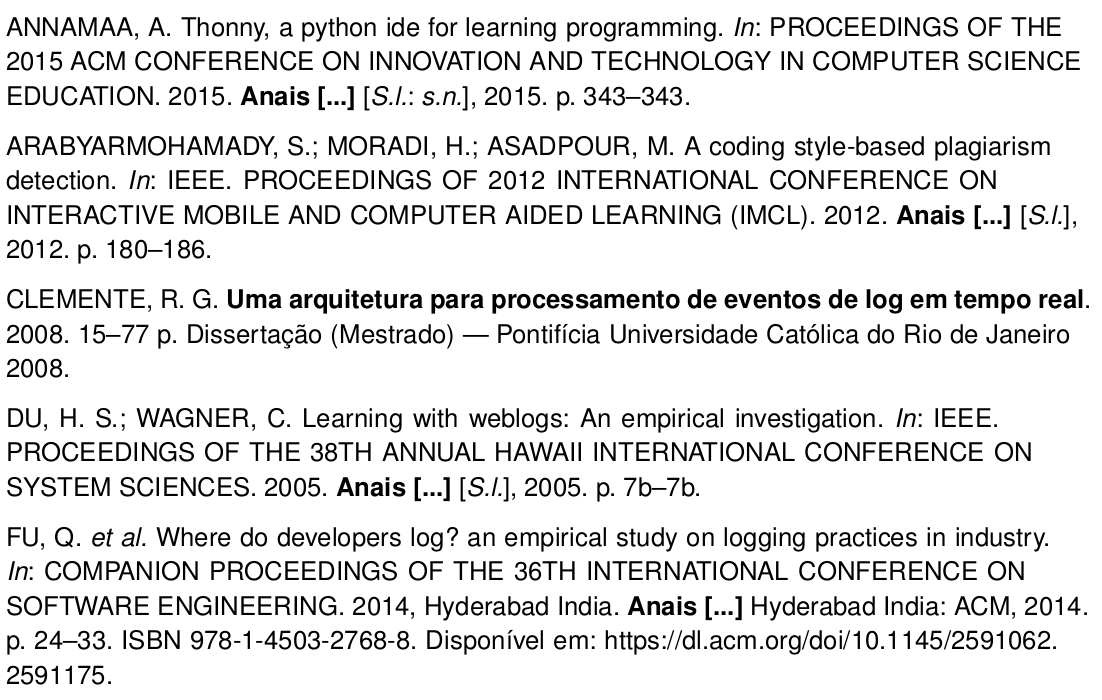
\includegraphics[scale=0.3]{ref0}
\end{frame}
\begin{frame}{Referências}
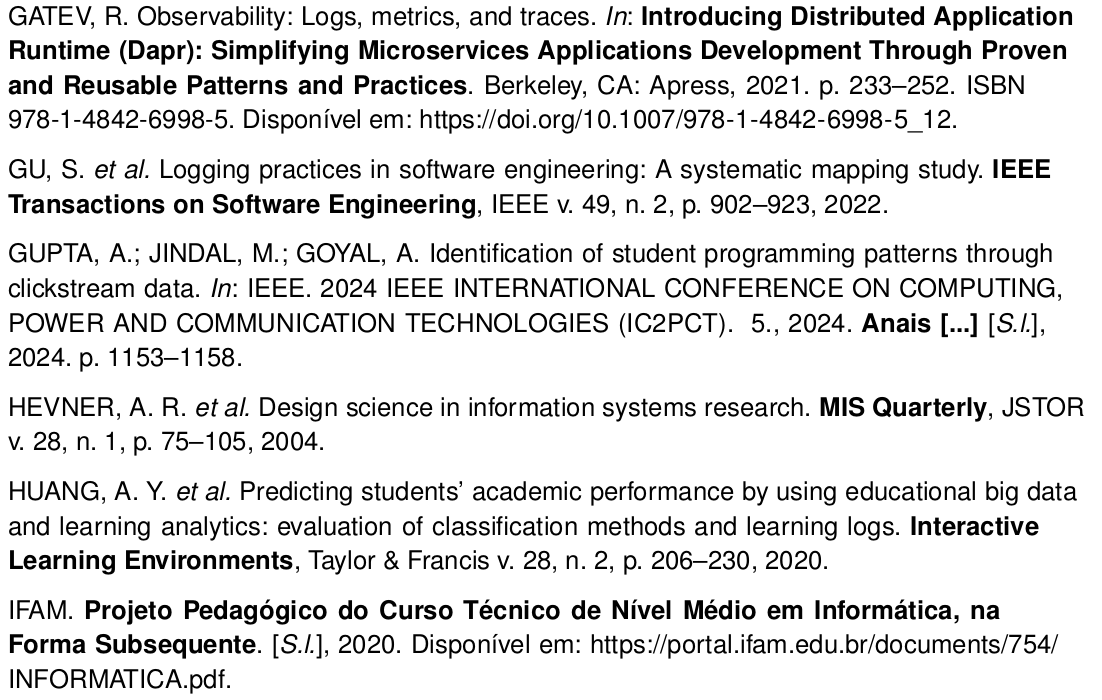
\includegraphics[scale=0.3]{ref1}
\end{frame}
\begin{frame}{Referências}

\includegraphics[scale=0.35]{ref2}
\end{frame}
\begin{frame}{Referências}
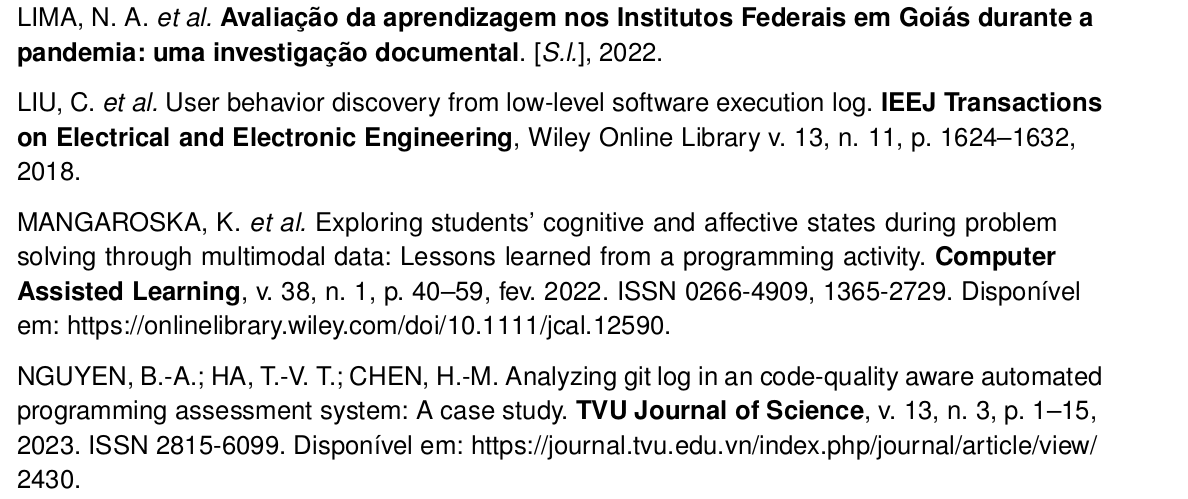
\includegraphics[scale=0.35]{ref3}
\end{frame}
\begin{frame}{Referências}
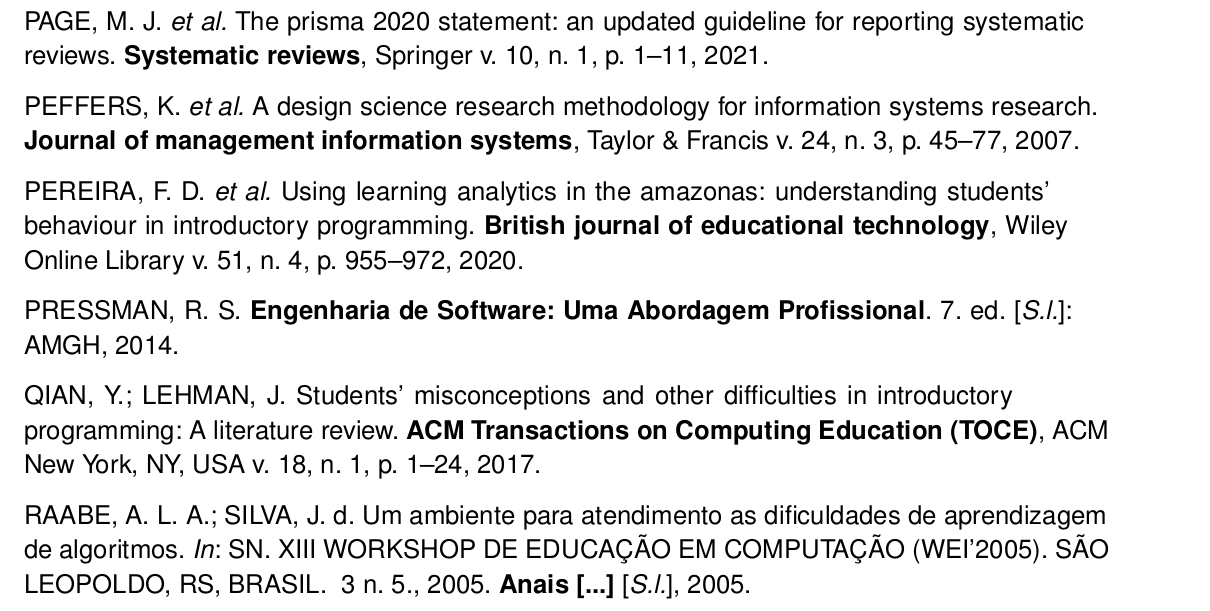
\includegraphics[scale=0.35]{ref4}
\end{frame}
\begin{frame}{Referências}
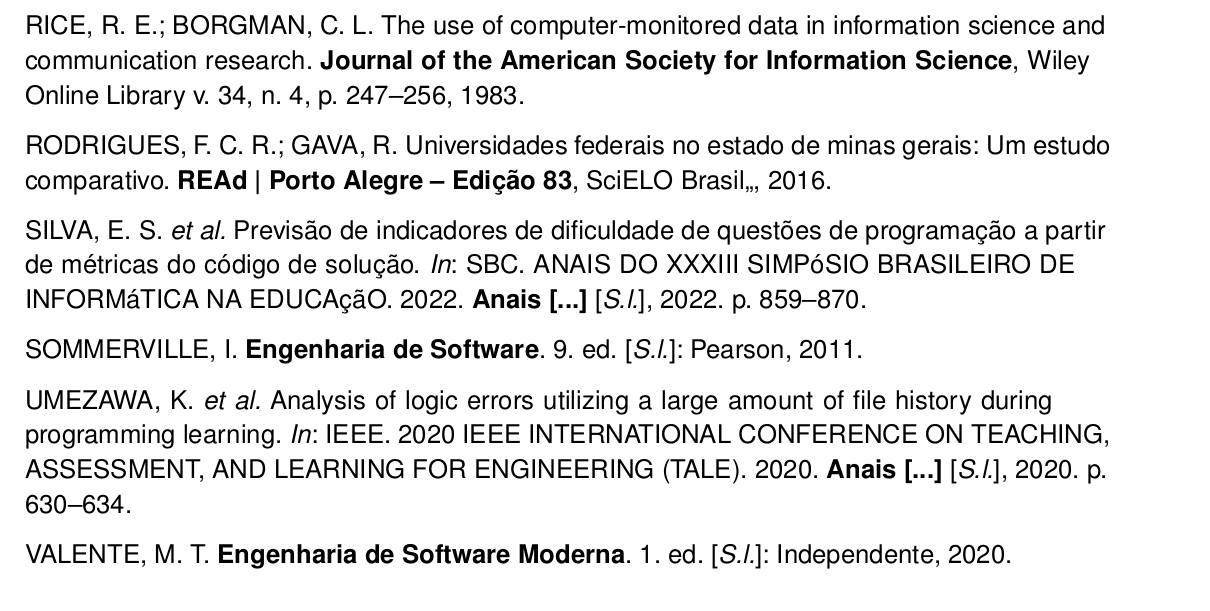
\includegraphics[scale=0.35]{ref5}
\end{frame}
\begin{frame}{Referências}
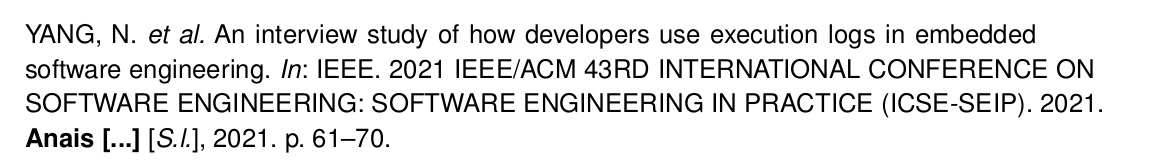
\includegraphics[scale=0.35]{ref6}
\end{frame}
\section{Agradecimentos}
\begin{frame}{Obrigado!}
%    \centering
%    \vspace*{0.5cm}
%    
%    {\Huge \textbf{Obrigado pela atenção!}}
%    
%    \vspace{1.2cm}
%    
%    % --- LINHA SUPERIOR: Trajetória Acadêmico-Profissional ---
%    \textbf{\footnotesize Minha trajetória}
%    
%    \vspace{0.3cm}
    
    \begin{columns}[c]
        % Alma Mater
        \column{0.33\textwidth}
        \centering
        
\includegraphics[height=2cm]{uft.jpeg} \\
        
        
        % Instituição de Trabalho
        \column{0.33\textwidth}
        \centering
        
\includegraphics[height=2cm]{ifam.png} \\
        
        % Universidade Atual (Mestrado)
        \column{0.33\textwidth}
        \centering
        
\includegraphics[height=1.1cm]{logoPPGCA.png} \\
        %\includegraphics[height=0.6cm]{sigla_mestrado.png} \\
        
    \end{columns}
    
    \vspace{1in}
    
    % --- LINHA INFERIOR: Produção Científica (Destaque) ---
   % \textbf{\footnotesize Produção desta pesquisa}
    
%    %\vspace{0.3cm}
%    \centering
    \begin{columns}[c]
        \column{0.33\textwidth}
        \column{0.33\textwidth}
        \centering
        
\includegraphics[height=2cm]{logado.jpeg}      %   \scriptsize \textbf{LOGADO} \\
      %  \tiny Artefato de pesquisa
        \column{0.33\textwidth}
    \end{columns}
    
%    \vspace{1cm}
%    
%    \footnotesize
%    \textbf{Seu Nome} • Qualificação de Mestrado • \today
\end{frame}
%\begin{frame}{Resultados}
%
%\begin{itemize}
%    \item Resultados 1
%    \item Resultados 2
%\end{itemize}
%
%\begin{block}{Bloco de destaque}
%    \begin{itemize}
%        \item Item 1
%        \item Item 2
%        \item Item 3
%        \item Item 3
%    \end{itemize}
%\end{block}

%\end{frame}

%%%%%%%%%%%%%%%%%%%%%%%%%%%%%%%%%%%%%%%%%%%%%%%%%%%%%%%%%%%%%

\end{document}
